\documentclass{standalone}
\usepackage{tikz}
\begin{document}
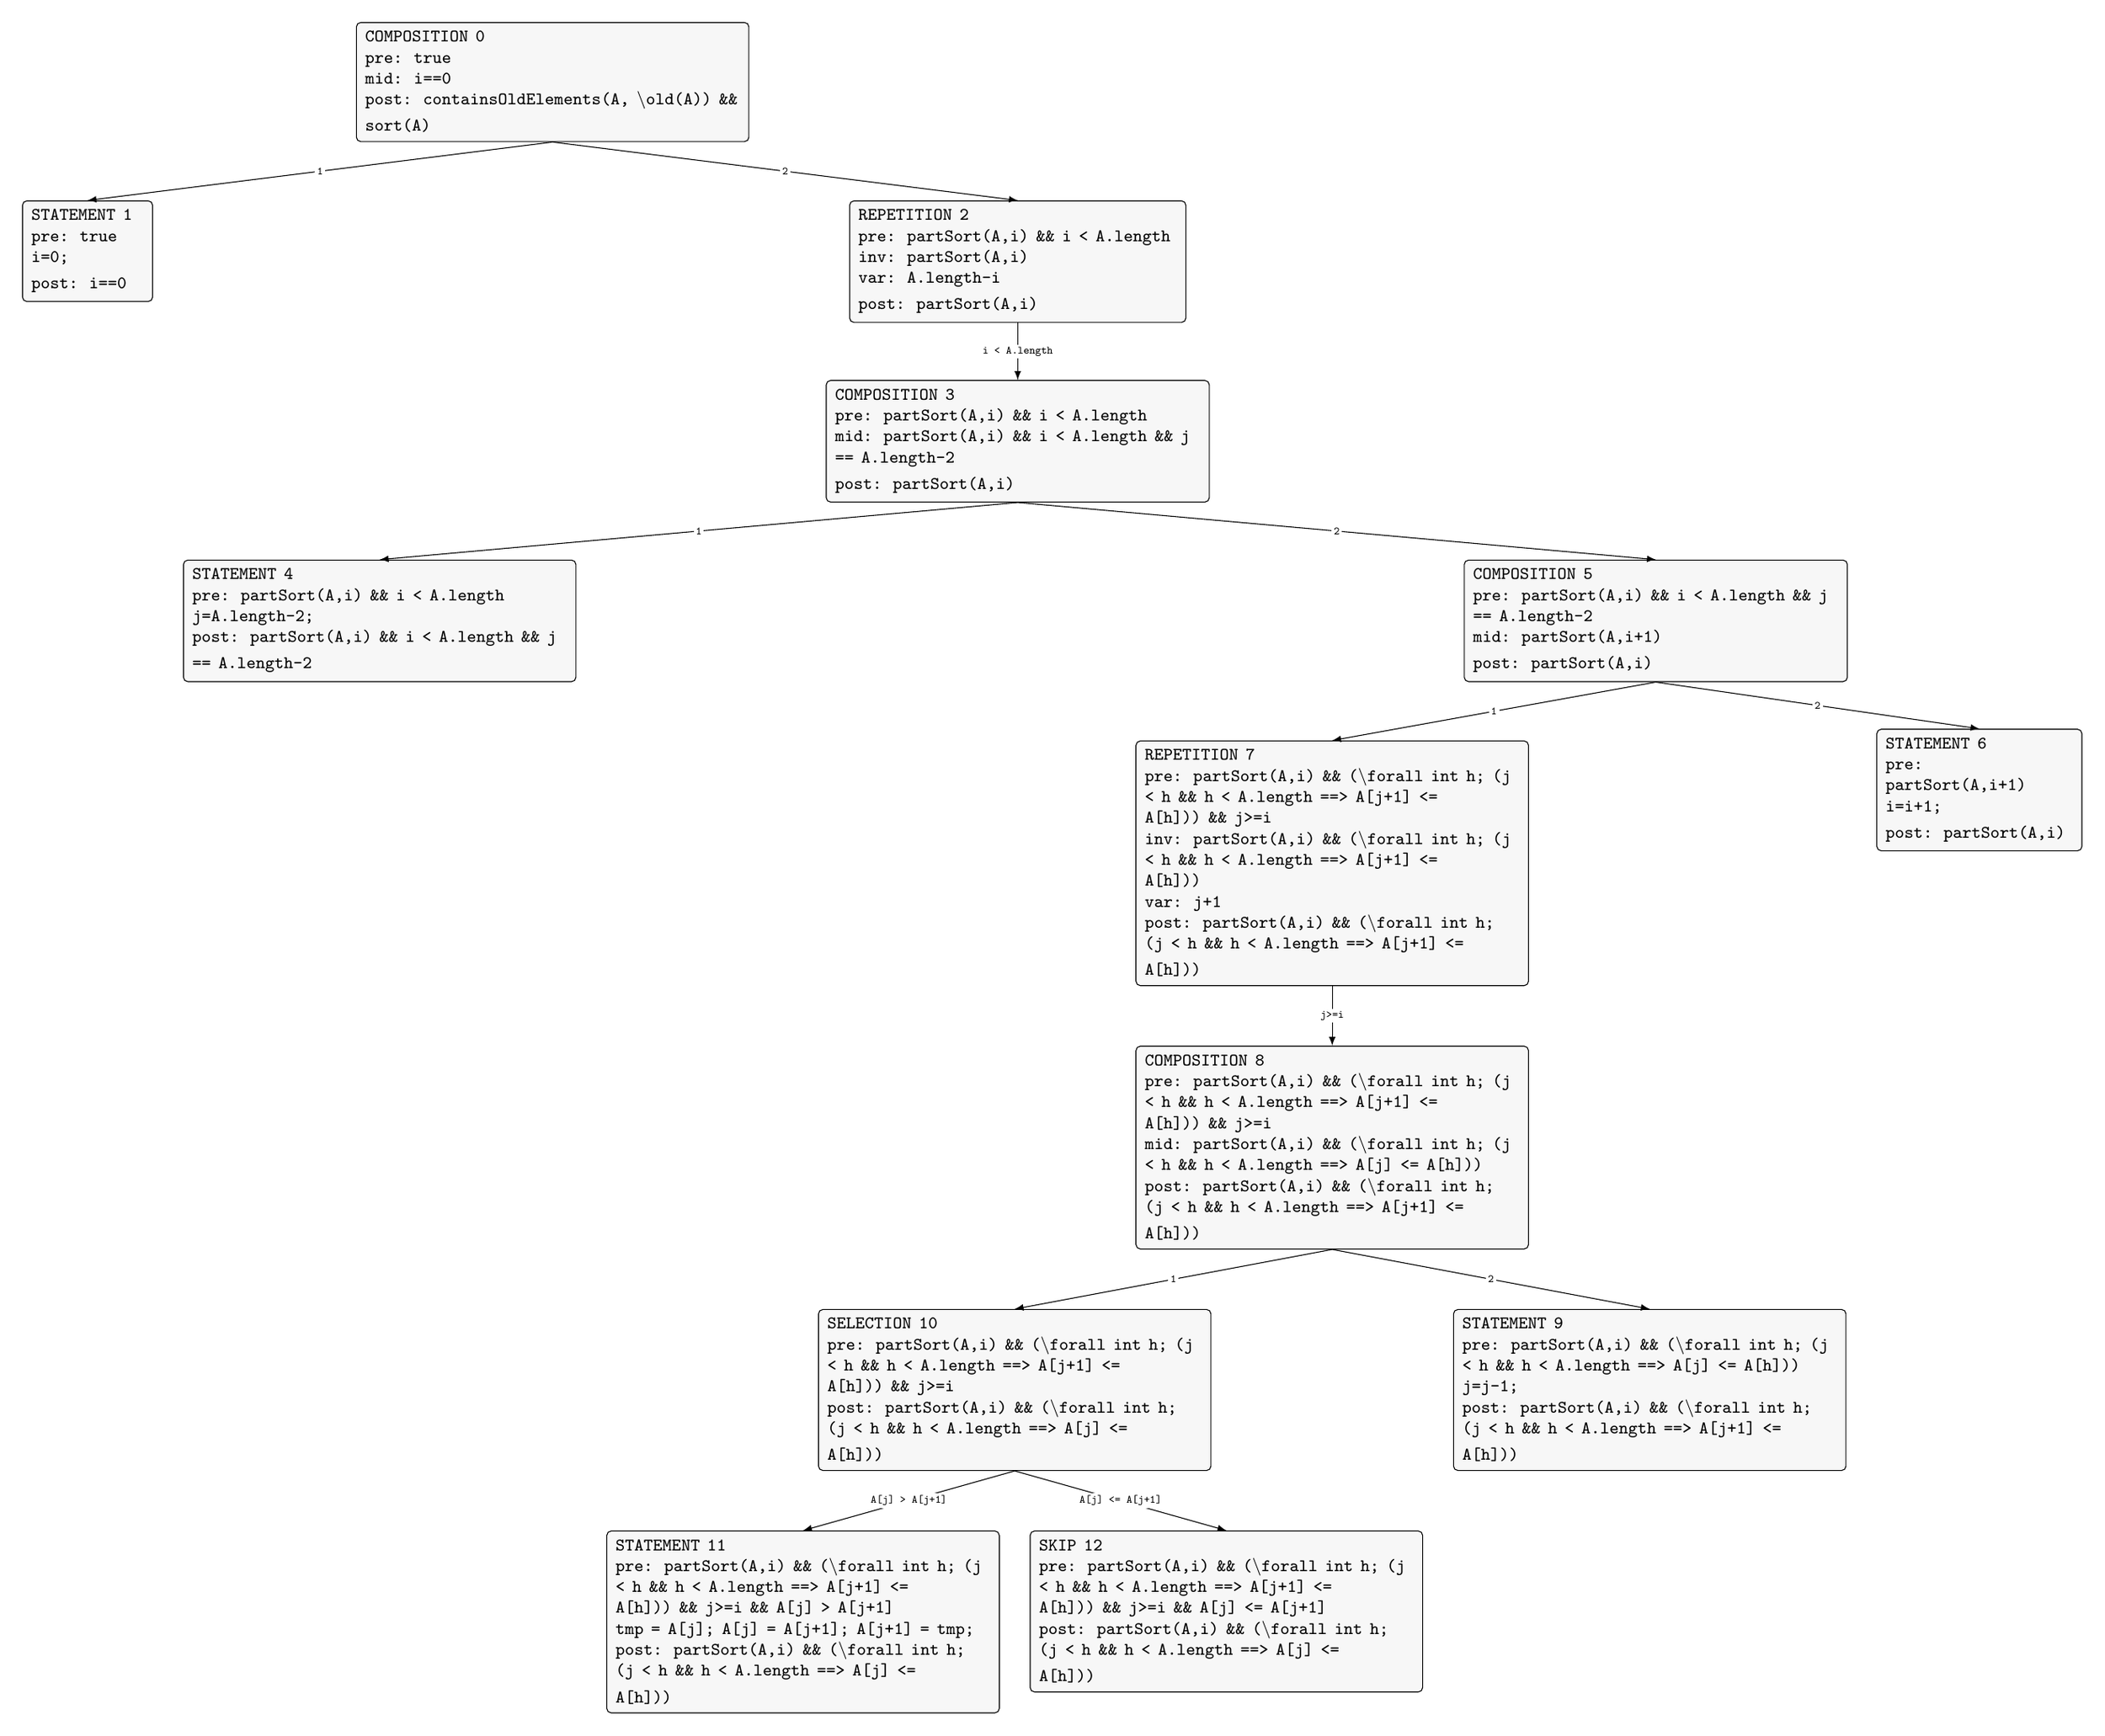
\begin{tikzpicture}[
  cbcnode/.style={draw, rounded corners=2pt, align=left, inner sep=4.0pt,
                  fill=black!3, line width=0.4pt},
  cbcedge/.style={draw, -latex, line width=0.4pt},
  cbclabel/.style={font=\tiny\ttfamily, fill=white, inner sep=1pt},
]
  \node[cbcnode, text width=170.002pt] (n81872) at (240.440pt,-27.750pt) {\footnotesize\ttfamily COMPOSITION  0\\pre: true\\mid: i==0\\post: containsOldElements(A, \textbackslash old(A)) \&\&\\  sort(A)};
  \node[cbcnode, text width=51.001pt] (n19696) at (29.500pt,-104.500pt) {\footnotesize\ttfamily STATEMENT  1\\pre: true\\i=0;\\post: i==0};
  \draw[cbcedge] (n81872.south) -- (n19696.north) node[cbclabel,midway]{1};
  \node[cbcnode, text width=144.502pt] (n19824) at (451.381pt,-109.250pt) {\footnotesize\ttfamily REPETITION  2\\pre: partSort(A,i) \&\& i < A.length\\inv: partSort(A,i)\\var: A.length-i\\post: partSort(A,i)};
  \node[cbcnode, text width=165.752pt] (n20336) at (451.381pt,-190.750pt) {\footnotesize\ttfamily COMPOSITION  3\\pre: partSort(A,i) \&\& i < A.length\\mid: partSort(A,i) \&\& i < A.length \&\& j\\  == A.length-2\\post: partSort(A,i)};
  \node[cbcnode, text width=170.002pt] (n20272) at (162.002pt,-272.250pt) {\footnotesize\ttfamily STATEMENT  4\\pre: partSort(A,i) \&\& i < A.length\\j=A.length-2;\\post: partSort(A,i) \&\& i < A.length \&\& j\\  == A.length-2};
  \draw[cbcedge] (n20336.south) -- (n20272.north) node[cbclabel,midway]{1};
  \node[cbcnode, text width=165.752pt] (n20976) at (740.759pt,-272.250pt) {\footnotesize\ttfamily COMPOSITION  5\\pre: partSort(A,i) \&\& i < A.length \&\& j\\  == A.length-2\\mid: partSort(A,i+1)\\post: partSort(A,i)};
  \node[cbcnode, text width=170.002pt] (n21040) at (594.007pt,-382.250pt) {\footnotesize\ttfamily REPETITION  7\\pre: partSort(A,i) \&\& (\textbackslash forall int h; (j\\  < h \&\& h < A.length ==> A[j+1] <=\\  A[h])) \&\& j>=i\\inv: partSort(A,i) \&\& (\textbackslash forall int h; (j\\  < h \&\& h < A.length ==> A[j+1] <=\\  A[h]))\\var: j+1\\post: partSort(A,i) \&\& (\textbackslash forall int h;\\  (j < h \&\& h < A.length ==> A[j+1] <=\\  A[h]))};
  \node[cbcnode, text width=170.002pt] (n21232) at (594.007pt,-511.250pt) {\footnotesize\ttfamily COMPOSITION  8\\pre: partSort(A,i) \&\& (\textbackslash forall int h; (j\\  < h \&\& h < A.length ==> A[j+1] <=\\  A[h])) \&\& j>=i\\mid: partSort(A,i) \&\& (\textbackslash forall int h; (j\\  < h \&\& h < A.length ==> A[j] <= A[h]))\\post: partSort(A,i) \&\& (\textbackslash forall int h;\\  (j < h \&\& h < A.length ==> A[j+1] <=\\  A[h]))};
  \node[cbcnode, text width=170.002pt] (n21808) at (450.006pt,-621.250pt) {\footnotesize\ttfamily SELECTION  10\\pre: partSort(A,i) \&\& (\textbackslash forall int h; (j\\  < h \&\& h < A.length ==> A[j+1] <=\\  A[h])) \&\& j>=i\\post: partSort(A,i) \&\& (\textbackslash forall int h;\\  (j < h \&\& h < A.length ==> A[j] <=\\  A[h]))};
  \node[cbcnode, text width=170.002pt] (n21488) at (354.004pt,-726.500pt) {\footnotesize\ttfamily STATEMENT  11\\pre: partSort(A,i) \&\& (\textbackslash forall int h; (j\\  < h \&\& h < A.length ==> A[j+1] <=\\  A[h])) \&\& j>=i \&\& A[j] > A[j+1]\\tmp = A[j]; A[j] = A[j+1]; A[j+1] = tmp;\\post: partSort(A,i) \&\& (\textbackslash forall int h;\\  (j < h \&\& h < A.length ==> A[j] <=\\  A[h]))};
  \draw[cbcedge] (n21808.south) -- (n21488.north) node[cbclabel,midway]{A[j] > A[j+1]};
  \node[cbcnode, text width=170.002pt] (n21680) at (546.007pt,-721.750pt) {\footnotesize\ttfamily SKIP  12\\pre: partSort(A,i) \&\& (\textbackslash forall int h; (j\\  < h \&\& h < A.length ==> A[j+1] <=\\  A[h])) \&\& j>=i \&\& A[j] <= A[j+1]\\post: partSort(A,i) \&\& (\textbackslash forall int h;\\  (j < h \&\& h < A.length ==> A[j] <=\\  A[h]))};
  \draw[cbcedge] (n21808.south) -- (n21680.north) node[cbclabel,midway]{A[j] <= A[j+1]};
  \draw[cbcedge] (n21232.south) -- (n21808.north) node[cbclabel,midway]{1};
  \node[cbcnode, text width=170.002pt] (n55728) at (738.009pt,-621.250pt) {\footnotesize\ttfamily STATEMENT  9\\pre: partSort(A,i) \&\& (\textbackslash forall int h; (j\\  < h \&\& h < A.length ==> A[j] <= A[h]))\\j=j-1;\\post: partSort(A,i) \&\& (\textbackslash forall int h;\\  (j < h \&\& h < A.length ==> A[j+1] <=\\  A[h]))};
  \draw[cbcedge] (n21232.south) -- (n55728.north) node[cbclabel,midway]{2};
  \draw[cbcedge] (n21040.south) -- (n21232.north) node[cbclabel,midway]{j>=i};
  \draw[cbcedge] (n20976.south) -- (n21040.north) node[cbclabel,midway]{1};
  \node[cbcnode, text width=85.001pt] (n55024) at (887.511pt,-349.000pt) {\footnotesize\ttfamily STATEMENT  6\\pre: partSort(A,i+1)\\i=i+1;\\post: partSort(A,i)};
  \draw[cbcedge] (n20976.south) -- (n55024.north) node[cbclabel,midway]{2};
  \draw[cbcedge] (n20336.south) -- (n20976.north) node[cbclabel,midway]{2};
  \draw[cbcedge] (n19824.south) -- (n20336.north) node[cbclabel,midway]{i < A.length};
  \draw[cbcedge] (n81872.south) -- (n19824.north) node[cbclabel,midway]{2};
\end{tikzpicture}
\end{document}
